%%%%%%%%%%%%%%%%%%%%%%%%%%%%%%%%%%%%%%%%%
% University Assignment Title Page 
% LaTeX Template
% Version 1.0 (27/12/12)
%
% This template has been downloaded from:
% http://www.LaTeXTemplates.com
%
% Original author:
% WikiBooks (http://en.wikibooks.org/wiki/LaTeX/Title_Creation)
%
% License:
% CC BY-NC-SA 3.0 (http://creativecommons.org/licenses/by-nc-sa/3.0/)
% 
% Instructions for using this template:
% This title page is capable of being compiled as is. This is not useful for 
% including it in another document. To do this, you have two options: 
%
% 1) Copy/paste everything between \begin{document} and \end{document} 
% starting at \begin{titlepage} and paste this into another LaTeX file where you 
% want your title page.
% OR
% 2) Remove everything outside the \begin{titlepage} and \end{titlepage} and 
% move this file to the same directory as the LaTeX file you wish to add it to. 
% Then add \input{./title_page_1.tex} to your LaTeX file where you want your
% title page.
%
%%%%%%%%%%%%%%%%%%%%%%%%%%%%%%%%%%%%%%%%%
%\title{Title page with logo}
%----------------------------------------------------------------------------------------
%	PACKAGES AND OTHER DOCUMENT CONFIGURATIONS
%----------------------------------------------------------------------------------------

\documentclass[12pt,technote]{IEEEtran}
\usepackage[english]{babel}
\usepackage[utf8x]{inputenc}
\usepackage{amsmath}
\usepackage{graphicx}
\usepackage{float}
\usepackage[colorinlistoftodos]{todonotes}

% Tables
\usepackage{multirow}

\begin{document}

\newcommand{\HRule}{\rule{\linewidth}{0.5mm}} % Defines a new command for the horizontal lines, change thickness here

\begin{center} % Center everything on the page
 
%----------------------------------------------------------------------------------------
%	HEADING SECTIONS
%----------------------------------------------------------------------------------------

\textsc{\small Università degli studi di Milano-Bicocca}\\[1cm] % Name of your university/college
\textsc{\Large Data and Text Mining }\\[0.3cm] % Major heading such as course name
\textsc{Final Project, June 2020}\\[0.1cm] % Minor heading such as course title

%----------------------------------------------------------------------------------------
%	TITLE SECTION
%----------------------------------------------------------------------------------------

\HRule \\[0.6cm]
{ \huge Cervical cancer risk exploratory study}\\ % Title of your document
\HRule \\[1.0cm]
 
%----------------------------------------------------------------------------------------
%	AUTHOR SECTION
%----------------------------------------------------------------------------------------

\large
\emph{Author:}\\
Antonio Vivace - 793509 a.vivace1@campus.unimib.it \\[1cm] % Your name

\end{center}

\begin{abstract}

Cervical Cancer is one of the most treatable cancers when diagnosed at early stages. Yet, it killed 311000 women in 2018 and it's still the fourth cause of death from cancers in women, the second most common in developing areas, mainly because of the economic cost and the difficulties in implementing effectives screening programmes. Data Mining provides robust tools to verify the known causal relations and assess risk factors from medical datasets. Classification models can then exploit this scenario to help identifying groups of population at higer risk to improve planning of screening programmes.



\end{abstract}

\section{Introduction}

This year in the US, there will be an estimated 13800 new cases of Cervical cancer. 4290 will be deadly \cite{acs}.
Worldwide, this type of cancer causes makes up 8\% of the total cancer cases and deaths. It's the fourth (second in developing countries \cite{Catarino2015}) cause of death from cancer in women.
A lot of progress has been made, and nowadays it is one of the most curable: when diagnosed and treated at the earliest stages, the five-year survival rate can reach 95\% \cite{cruk}.

In this work, we investigate the possibility of classifying high-risk patients from demographic and other medical data, but excluding the results of other related exams.

\begin{figure}
    \centerline{
        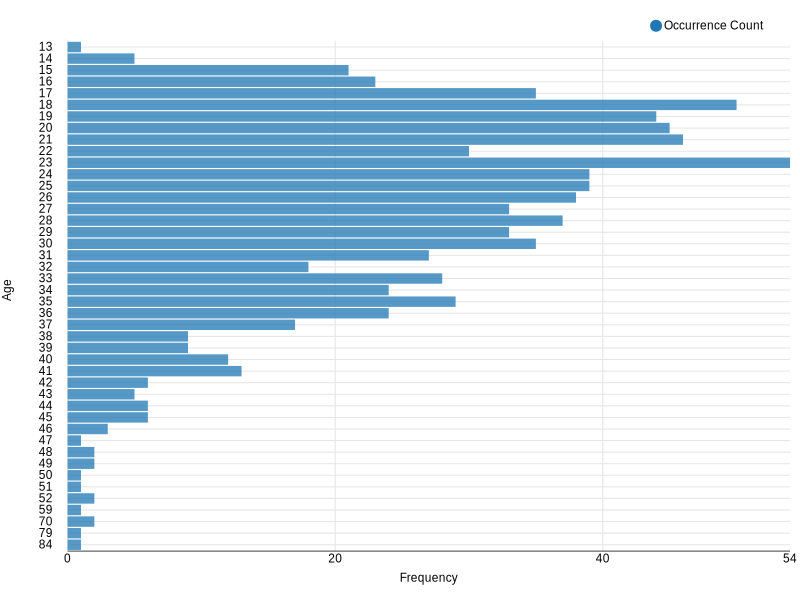
\includegraphics[width=0.4\paperwidth]{figures/age_dist.pdf}}
    \caption{Age distribution}
    \label{age_distribution}
\end{figure}
\paragraph{Known causal relations}

HPV causal relation with the cervical cancer has been documented beyond reasonable doubt \cite{Bosch2002}. Additionally, Human papilloma virus (HPV) infection is necessary for the development of CIN, the abnormal growth of cells on the surface of the cervix, indicating a potentially precancerous transformation of cells of the cervix \cite{kumar2017robbins}.

Risk factors include smoking, \cite{Collins2010} early age at the first sexual intercourse and early pregnancies.

\section{Dataset}

The dataset was collected at 'Hospital Universitario de Caracas' in Caracas, Venezuela.

36 attributes describe demographic informations, sexual activity and frequency, pregnancies, age, smoke addiction, usage of contraceptives and diagnosed Sexualy Transmitted Diseases of 858 women patients.

\begin{figure}
    \centerline{
        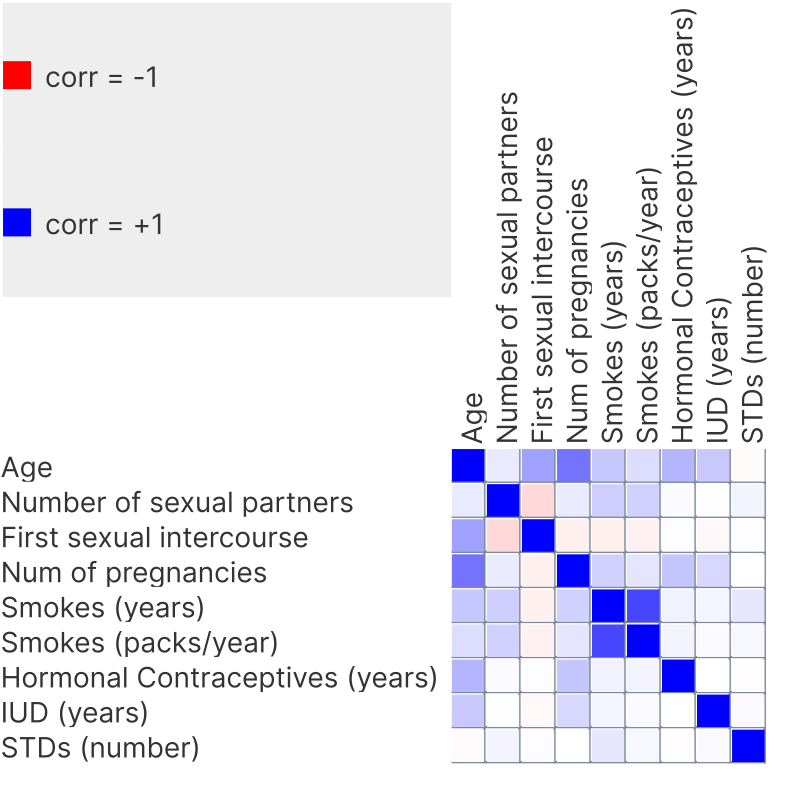
\includegraphics[width=0.3\paperwidth]{figures/corr.png}}
    \caption{Correlation Matrix on the numeric attributes of the starting dataset}
    \label{correlation_matrix}
\end{figure}


The missing values are due to the decision of the patients to not disclose those details because of privacy concerns.

We'll introduce some context and clarifications on the attributes significance to outline the relationship with the disease:

\begin{itemize}
    \item \textbf{Hormonal Contraceptives} indicates if the patient uses \textit{hormonal} contraceptives. \textbf{IUD} indicates the usage of the Intra Uterine contraceptive Device.
    \item \textbf{STDs} indicates if the patient had at least one Sexually Transmitted Disease. It's positive when at least one of the STDs:condylomatosis, STDs:cervical condylomatosis, STDs:vaginal condylomatosis, STDs:vulvo-perineal condylomatosis, STDs:syphilis, STDs:pelvic inflammatory disease, STDs:genital herpes, STDs:molluscum contagiosum, STDs:AIDS, STDs:HIV, STDs:Hepatitis, STDs:HPV attributes is positive.
    \item \textbf{STDs:HPV} indicates if the patient is infected by the \textit{Human Papilloma Virus}.
    \item \textbf{Dx:HPV} reveals if the patient was already diagnosed with HPV in the past.
    \item \textbf{Dx:Cancer} is positive if the patient already had cancer. It is not clear if this refers to Breast Cancer, as diagnosable by the Oncotype DX test or any type of cancer. The original paper presenting this dataset has no additional information on this \cite{articleUCI}.
    \item \textbf{Dx:CIN} indicates if the patient was affected by Cervical intraepithelial neoplasia (CIN).
    \item \textbf{Dx} is positive if at least one of the Dx variables is positive.
    \item \textbf{Hinselmann} and \textbf{Citology} are two (complementary \cite{Duncan2004}) tests to detect Cervical Cancer. \textbf{Schiller} is another test able to identify abnormal areas to be biopsied and examined.
    \item \textbf{Biopsy} is a medical procedure providing a confirmation of the diagnosis through a \textit{colposcopy}, a magnified visual inspection of the cervix. This attribute has been chosen as our target.
\end{itemize}

\section{The Methodological Approach}

\begin{figure}
    \centerline{
        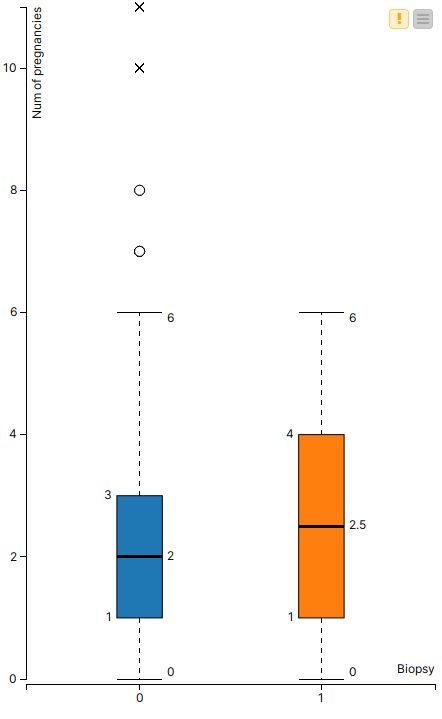
\includegraphics[width=0.25\paperwidth]{figures/boxplot1.png}}
    \caption{Biopsy VS number of pregnancies conditional box plot}
    \label{cond_box_plot}
\end{figure}

\subsection{Exploration}

\begin{figure}
    \centerline{
        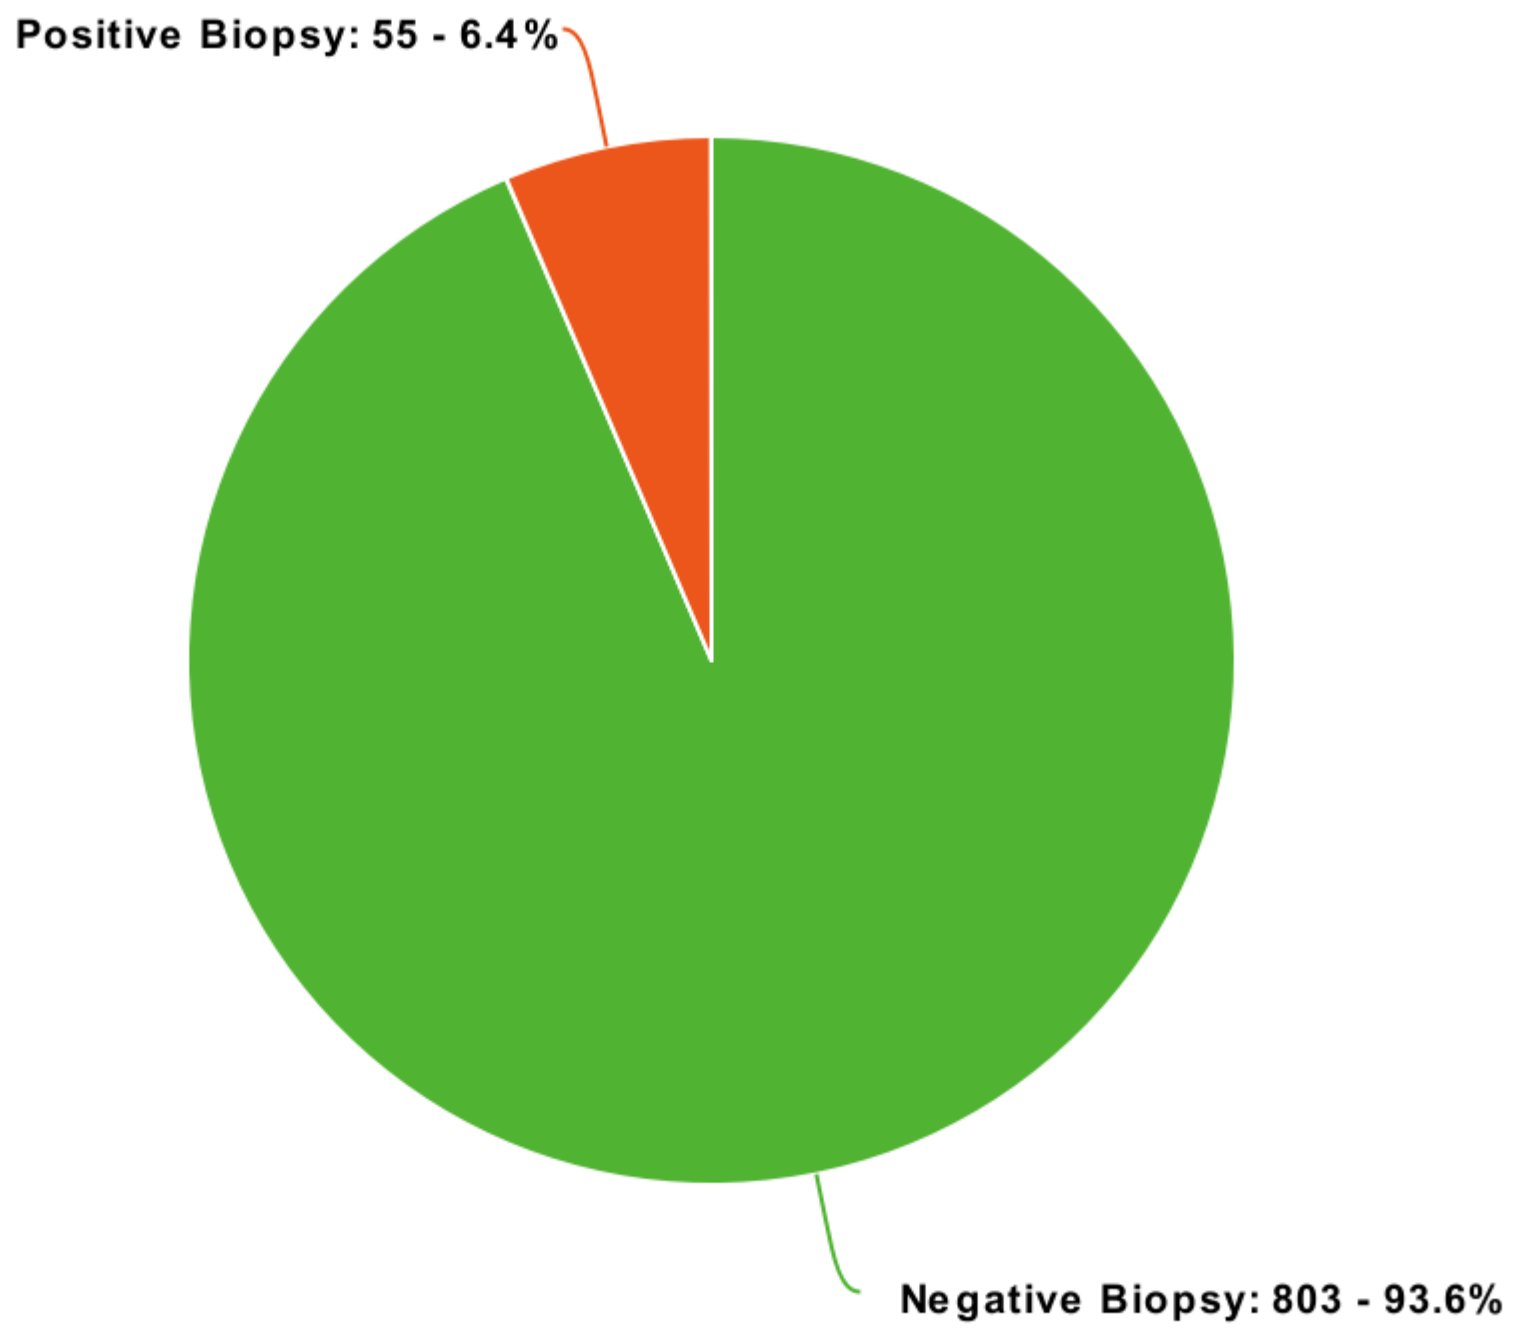
\includegraphics[width=0.3\paperwidth]{figures/class_unbalance.png}}
    \caption{Unbalanced biopsy distribution}
    \label{unbalanced_biopsy}
\end{figure}

The target class is highly unbalanced (Figure \ref{unbalanced_biopsy}), with only 6.4\% of positive values.

The main statistical descriptors have been computed and studied. Age distribution is shown in Figure \ref{age_distribution}: the majority of the instances refers to young women (younger than 15 and older than 38 years old can be considered outliers). Almost all of them had at least one pregnancy (98,1\%).

\subsection{Feature Selection}

We decided to exclude the other tests (\textbf{Hinselmann}, \textbf{Citology}, \textbf{Schiller}) since, by conception, they share a similar purpose with the target \textbf{Biopsy}.

\textbf{STDs:Time since first diagnosis} and \textbf{STDs:Time since last diagnosis} are missing in more than 90\% of the records and were filtered out.

\textbf{STDs:cervical condylomatosis} and \textbf{STDs:AIDS}, \textbf{STDs:pelvic inflammatory disease}, \textbf{STDs: molluscum contagiosum}, \textbf{STDs:Hepatitis B} and \textbf{STDs:HPV} were removed because they had more than 99.995\% negative (or missing) values.

Finally, \textbf{Smokes}, \textbf{Hormonal Contraceptives} and \textbf{IUD} were removed because the correspondings "Years" attributes already provide these informations.

\subsection{Missing Values}

Missing values have been imputed with the conditioned average value per Age class. 5 Age classes with same frequency have been created, using the \textit{Equal frequency unsupervised discretization method}: 13-19, 19-23, 23,28, 28-34, 34-84.

Finally, to avoid inv the Z-Score Normalization has been applied.

After this steps, the dataset has 20 normalized attributes and no missing values:

\begin{itemize}
    \item Age
    \item Number of sexual partners
    \item First sexual intercourse
    \item Num of pregnancies
    \item Smokes (years)
    \item Smokes (packs/year)
    \item Hormonal Contraceptives (years)
    \item IUD (years)
    \item STDs (number)
    \item STDs:condylomatosis
    \item STDs:vaginal condylomatosis
    \item STDs:vulvo-perineal condylomatosis
    \item STDs:syphilis
    \item STDs:genital herpes
    \item STDs:HIV
    \item STDs: Number of diagnosis
    \item Dx:Cancer
    \item Dx:CIN
    \item Dx:HPV
    \item Biopsy
\end{itemize}

\subsection{Correlation}

Some mentioned causal relations can be seen through this step: early age at first sexual intercourse, number of pregnancies.

\textbf{Dx} is not clearly correlated with Biopsy, probably because the type of cancer it refers to it's unrelated (Breast).

The other tests (\textbf{Hinselmann}, \textbf{Citology}, \textbf{Schiller}) are obviously very correlated with Biopsy (Figure \ref{correlation_matrix}).

\begin{figure}
    \centerline{
        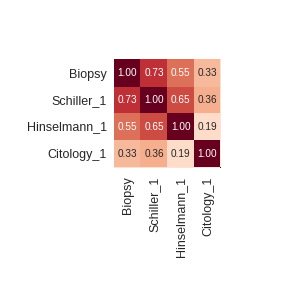
\includegraphics[width=0.25\paperwidth]{figures/exams_corr.png}}
    \caption{Correlation matrix of Cervical Cancer exams}
    \label{cond_box_plot}
\end{figure}

Even if it's been shown that smoking it's a risk factor for CIN, the potential initial step of a Cervical Cancer, this is not visibile in this dataset.

\subsection{Class imbalance}

Two approaches have been experimented to handle this issue: oversampling with SMOTE (\cite{Chawla2011}) and the usage of cost-sensitive Random Forest classificator.

To avoid inflating metrics, SMOTE oversampling has been applied only on the training sets.

The cost-sensitive model makes use of the cost matrix shown in Table \ref{table:confusion_matrix}, to try to minimize the False Negative Rate. The cost given to False Negatives (ignoring when a cancer is present) is 10 times the cost of False Positives (flagging a cancer even when it's not true).

\begin{table}[]
    \centering
    \begin{tabular}{lllll}
                                             &          &                                           &          & \\
        \multirow{2}{*}{}                    &          & \multicolumn{2}{l}{\textbf{Ground Truth}} &            \\
                                             &          & Positive                                  & Negative & \\
        \multirow{2}{*}{\textbf{Prediction}} & Positive & 1.0                                       & 1.0       & \\
                                             & Negative & 10.0                                      & 1.0       &
    \end{tabular}
    \caption{Cost Matrix}
    \label{table:confusion_matrix}
\end{table}

\begin{table}[]
\begin{tabular}{ll}
Attribute                          & Importance          \\
First sexual intercourse           & 2.5964373464373462  \\
Hormonal Contraceptives (years)    & 2.126984126984127   \\
Number of sexual partners          & 1.593911719939117   \\
Age                                & 1.196969696969697   \\
Num of pregnancies                 & 1.0419717887154862  \\
STDs (number)                      & 0.8303292827102351  \\
Dx:HPV                             & 0.8073291050035236  \\
Dx:Cancer                          & 0.720280437756498   \\
STDs: Number of diagnosis          & 0.4703452178834182  \\
Smokes (years)                     & 0.38181818181818183 \\
Smokes (packs/year)                & 0.37965816755393667 \\
IUD (years)                        & 0.3663967611336032  \\
STDs:HIV                           & 0.35227272727272724 \\
STDs:vulvo-perineal condylomatosis & 0.28707870787078704 \\
STDs:condylomatosis                & 0.2577920377160817  \\
STDs:syphilis                      & 0.152191894127378   \\
Dx:CIN                             & 0.14195402298850573 \\
STDs:vaginal condylomatosis        & 0.08712121212121213 \\
STDs:genital herpes                & 0.05130718954248366
\end{tabular}
\caption{Feature importance, according to the Random Forest (SMOTE) model (all levels).}
\label{table:feature_importance}

\end{table}

\subsection{Classification}

The following models have been tested, using a 5-Fold stratified cross validation learning: Random Forest and Logistic Regression. The features used are the selected one, while the split dataset (1/3, 2/3) and oversampled ones are being (separately) used (SMOTE and cost matrix).

Overview of the different configuration tried:
\begin{enumerate}
    \item SMO with non-oversampled dataset (split 2/3 and 1/3)
    \item SMO with SMOTE oversampling
    \item Random Forest with non-oversampled dataset (split 2/3 and 1/3)
    \item Random Forest with SMOTE
    \item Random Forest with Cost Matrix
    \end{enumerate}

Higher number of folds are infeasible since the dataset is highly unbalanced. These metrics are computed and compared: Accuracy, Precision, Recall and F1 Score.

The trained Random Forest model is used to extract the importance (see Figure \ref{table:feature_importance}) of the attributes. This step is very informative and can be used as a feature selector for other models and can highlight risk factors.

Importance from the RandomForest model is computed from the Splits and Candidates values:

$$\text{Importance}_i = \frac{\text{splits}_i}{\text{candidates}_i} $$

Where i is the level. The KNIME implementations gives 3 levels and we sum them all.

\section{Results and conclusions}

Exploring medical datasets on can help validate the causal relations, but predicting a diagnosis without any targeted test or exam, having only partial information on behaviours related to risk factors is definitely a challenging task and we didn't get excellent results.

Perfomance of the classificators can appear unsatisfying, but this work provides a baseline where additional data and more complex ML tools can exploit additional (and less unbalanced) datasets. Furthermore, exploiting trained models to rank risk factors can help build more relevant datasets, providing guidelines on which values and aspects about patients should be investigated and mined.


On the other hand, classificators results improve drastically when tests targeted to the same disease are available. This is expected, as each of exam have large medical literature describing their accuracy and diagnosing power.

Oversampling medical data with SMOTE also didn't show any particular enhancement, as the instances are syntethic and tend to overrepresent particular patterns, thus confusing the classificators or not getting any improvement at all. The dataset also had a really low and unbalanced number of positive cases, on a already largely biased sample (Age distribution of patients, pregnancies).

Correctly evaluating the bias and the sample distribution from which the instances are sampled can also help in understanding how to handle the missing values. Here, our missing-imputation strategy keeps (and actually empowers) the bias, effectively supposing that if someone didn't answer, the truth should be similar to their peers (similar age, similar geographic provenience, ...). Since missing values weren't a minor issue, and they are due to privacy concerns, this is mostly a cultural consideration. A possible additional experimentation could be to change this approach.

However, the Correlation Analysis and the Feature importance extraction shows how the attributes related to known risk factors are popping out as the most important (\ref{table:feature_importance}), and reflect the known causal relations we mentioned. Having richer datasets, providing more complete details about the medical history of the patient could lead to more accurate results and could enable proper clustering of patient population, suggesting the ones subject to higher risks.

Furthermore, cultural details plays a fundamental role in sexual habits and STDs related issues, but these elements are non-trivial to tackle and proper factor in medical machine learning models. E.g., it's been shown that early age at the first sexual intercourse and early pregnancies are strongly \textit{interrelated} in most developing countries \cite{Louie2009}.

Bigger, richer and more complete datasets, including socio-economical and ethnic data on the patients could lead to intersting investigations and improve this strategy to highlight and cluster high-risk groups.

\bibliographystyle{IEEEtran}
\bibliography{references.bib}

\end{document}